\documentclass{article}\usepackage[]{graphicx}\usepackage[]{color}
%% maxwidth is the original width if it is less than linewidth
%% otherwise use linewidth (to make sure the graphics do not exceed the margin)
\makeatletter
\def\maxwidth{ %
  \ifdim\Gin@nat@width>\linewidth
    \linewidth
  \else
    \Gin@nat@width
  \fi
}
\makeatother

\definecolor{fgcolor}{rgb}{0.345, 0.345, 0.345}
\newcommand{\hlnum}[1]{\textcolor[rgb]{0.686,0.059,0.569}{#1}}%
\newcommand{\hlstr}[1]{\textcolor[rgb]{0.192,0.494,0.8}{#1}}%
\newcommand{\hlcom}[1]{\textcolor[rgb]{0.678,0.584,0.686}{\textit{#1}}}%
\newcommand{\hlopt}[1]{\textcolor[rgb]{0,0,0}{#1}}%
\newcommand{\hlstd}[1]{\textcolor[rgb]{0.345,0.345,0.345}{#1}}%
\newcommand{\hlkwa}[1]{\textcolor[rgb]{0.161,0.373,0.58}{\textbf{#1}}}%
\newcommand{\hlkwb}[1]{\textcolor[rgb]{0.69,0.353,0.396}{#1}}%
\newcommand{\hlkwc}[1]{\textcolor[rgb]{0.333,0.667,0.333}{#1}}%
\newcommand{\hlkwd}[1]{\textcolor[rgb]{0.737,0.353,0.396}{\textbf{#1}}}%

\usepackage{framed}
\makeatletter
\newenvironment{kframe}{%
 \def\at@end@of@kframe{}%
 \ifinner\ifhmode%
  \def\at@end@of@kframe{\end{minipage}}%
  \begin{minipage}{\columnwidth}%
 \fi\fi%
 \def\FrameCommand##1{\hskip\@totalleftmargin \hskip-\fboxsep
 \colorbox{shadecolor}{##1}\hskip-\fboxsep
     % There is no \\@totalrightmargin, so:
     \hskip-\linewidth \hskip-\@totalleftmargin \hskip\columnwidth}%
 \MakeFramed {\advance\hsize-\width
   \@totalleftmargin\z@ \linewidth\hsize
   \@setminipage}}%
 {\par\unskip\endMakeFramed%
 \at@end@of@kframe}
\makeatother

\definecolor{shadecolor}{rgb}{.97, .97, .97}
\definecolor{messagecolor}{rgb}{0, 0, 0}
\definecolor{warningcolor}{rgb}{1, 0, 1}
\definecolor{errorcolor}{rgb}{1, 0, 0}
\newenvironment{knitrout}{}{} % an empty environment to be redefined in TeX

\usepackage{alltt}
\usepackage[margin=0.5in]{geometry}





\IfFileExists{upquote.sty}{\usepackage{upquote}}{}
\begin{document}


\begin{knitrout}
\definecolor{shadecolor}{rgb}{0.969, 0.969, 0.969}\color{fgcolor}\begin{kframe}
\begin{alltt}
\hlstd{> }\hlkwd{set.seed}\hlstd{(}\hlnum{3}\hlstd{)}  \hlcom{# setting seed for reproducibility}
\hlstd{> }\hlstd{i} \hlkwb{<-} \hlnum{1}
\hlstd{> }\hlstd{N} \hlkwb{<-} \hlnum{10}\hlopt{^}\hlnum{5} \hlopt{-} \hlnum{1}  \hlcom{# N = number of simulations}
\hlstd{> }\hlstd{N2mat} \hlkwb{<-} \hlkwd{matrix}\hlstd{(}\hlnum{0}\hlstd{, N,} \hlnum{2}\hlstd{)}  \hlcom{# initialize N*2 matrix to all 0's}
\hlstd{> }\hlkwa{repeat} \hlstd{\{}
\hlstd{+ }    \hlstd{N2mat[i, ]} \hlkwb{<-} \hlkwd{sample}\hlstd{(}\hlnum{1}\hlopt{:}\hlnum{6}\hlstd{,} \hlnum{2}\hlstd{,} \hlkwc{replace} \hlstd{=} \hlnum{TRUE}\hlstd{)}
\hlstd{+ }    \hlkwa{if} \hlstd{(i} \hlopt{==} \hlstd{N)}
\hlstd{+ }        \hlkwa{break}
\hlstd{+ }    \hlstd{i} \hlkwb{<-} \hlstd{i} \hlopt{+} \hlnum{1}
\hlstd{+ }\hlstd{\}}
\hlstd{> }\hlstd{means} \hlkwb{<-} \hlkwd{apply}\hlstd{(N2mat,} \hlnum{1}\hlstd{, mean)}
\hlstd{> }\hlstd{T3} \hlkwb{<-} \hlkwd{table}\hlstd{(means)}
\hlstd{> }\hlstd{T3}
\end{alltt}
\begin{verbatim}
means
    1   1.5     2   2.5     3   3.5     4   4.5     5   5.5     6 
 2802  5523  8394 11138 13938 16552 13876 11202  8287  5576  2711 
\end{verbatim}
\end{kframe}
\end{knitrout}

The function \texttt{plot()} is applied to \texttt{T3} after dividing its contents by \texttt{N}.  The result, with a few embellishments, is presented in Figure \ref{c01PLOTMEANS}. 


\begin{figure}[!ht]
\centering
\begin{knitrout}
\definecolor{shadecolor}{rgb}{0.969, 0.969, 0.969}\color{fgcolor}
\includegraphics[width=.45\linewidth]{./figure/Color/c01PLOTMEANSfig-1} 

\end{knitrout}
\caption{Graphical representation of the relative frequency of each of the possible means from a simulation of throwing two dice 99,999 times \label{c01PLOTMEANS}}
\end{figure}

\begin{knitrout}
\definecolor{shadecolor}{rgb}{0.969, 0.969, 0.969}\color{fgcolor}\begin{kframe}
\begin{alltt}
\hlstd{> }\hlkwd{hist}\hlstd{(}\hlkwd{rnorm}\hlstd{(}\hlnum{10000}\hlstd{),} \hlkwc{col} \hlstd{=} \hlstr{"red"}\hlstd{)}
\end{alltt}
\end{kframe}
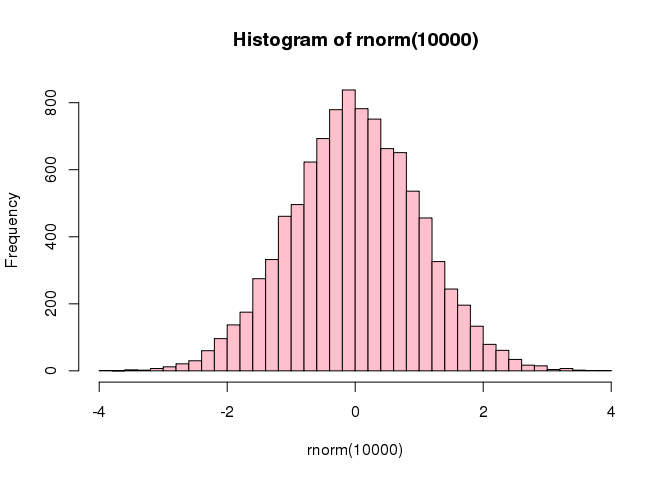
\includegraphics[width=\maxwidth]{./figure/Color/unnamed-chunk-1-1} 

\end{knitrout}

Green now:

\begin{knitrout}
\definecolor{shadecolor}{rgb}{0.969, 0.969, 0.969}\color{fgcolor}\begin{kframe}
\begin{alltt}
\hlstd{> }\hlkwd{hist}\hlstd{(}\hlkwd{rnorm}\hlstd{(}\hlnum{10000}\hlstd{),} \hlkwc{col} \hlstd{=} \hlstr{"green"}\hlstd{)}
\end{alltt}
\end{kframe}
\includegraphics[width=\maxwidth]{./figure/Color/unnamed-chunk-2-1} 

\end{knitrout}

\end{document}
